%%%%%%%%%%%%%%%%%%%%%%%%%%%%%%%%%%%%%%%%%
% Beamer Presentation
% LaTeX Template
% Version 1.0 (10/11/12)
%
% This template has been downloaded from:
% http://www.LaTeXTemplates.com
%
% License:
% CC BY-NC-SA 3.0 (http://creativecommons.org/licenses/by-nc-sa/3.0/)
%
%%%%%%%%%%%%%%%%%%%%%%%%%%%%%%%%%%%%%%%%%

\documentclass[t]{beamer}

\usepackage[english]{babel}
\usepackage[utf8]{inputenc}
\usepackage{hyperref}
\usepackage{verbatim}
\usepackage{listings}

%----------------------------------------------------------------------------------------
%	PACKAGES AND THEMES
%----------------------------------------------------------------------------------------

\mode<presentation> {

% The Beamer class comes with a number of default slide themes
% which change the colors and layouts of slides. Below this is a list
% of all the themes, uncomment each in turn to see what they look like.

%\usetheme{default}
%\usetheme{AnnArbor}
%\usetheme{Antibes}
%\usetheme{Bergen}
%\usetheme{Berkeley}
%\usetheme{Berlin}
%\usetheme{Boadilla}
%\usetheme{CambridgeUS}
%\usetheme{Copenhagen}
%\usetheme{Darmstadt}
%\usetheme{Dresden}
%\usetheme{Frankfurt}
%\usetheme{Goettingen}
%\usetheme{Hannover}
%\usetheme{Ilmenau}
%\usetheme{JuanLesPins}
%\usetheme{Luebeck}
%\usetheme{Madrid}
%\usetheme{Malmoe}
%\usetheme{Marburg}
%\usetheme{Montpellier}
%\usetheme{PaloAlto}
%\usetheme{Pittsburgh}
%\usetheme{Rochester}
%\usetheme{Singapore}
%\usetheme{Szeged}
\usetheme{Warsaw}

% As well as themes, the Beamer class has a number of color themes
% for any slide theme. Uncomment each of these in turn to see how it
% changes the colors of your current slide theme.

%\usecolortheme{albatross}
%\usecolortheme{beaver}
%\usecolortheme{beetle}
%\usecolortheme{crane}
%\usecolortheme{dolphin}
%\usecolortheme{dove}
%\usecolortheme{fly}
%\usecolortheme{lily}
%\usecolortheme{orchid}
%\usecolortheme{rose}
\usecolortheme{seagull}
%\usecolortheme{seahorse}
%\usecolortheme{whale}
%\usecolortheme{wolverine}

\usefonttheme{structuresmallcapsserif}

%\setbeamertemplate{footline} % To remove the footer line in all slides uncomment this line
%\setbeamertemplate{footline}[page number] % To replace the footer line in all slides with a simple slide count uncomment this line

%\setbeamertemplate{navigation symbols}{} % To remove the navigation symbols from the bottom of all slides uncomment this line
}


\usepackage{graphicx} % Allows including images
\usepackage{booktabs} % Allows the use of \toprule, \midrule and \bottomrule in tables



\lstdefinestyle{cpp}{
  language=C++,
  basicstyle=\ttfamily\footnotesize,  % Use small true type font
  showstringspaces=false,                 % Don't put marks in string spaces
  tabsize=2,                              % 5 spaces per tab
  escapeinside={@}{@},                % for invisible labels
  breaklines=true,
  breakatwhitespace=true,
  emptylines=1,
  texcl=true,
  escapechar=@,
  mathescape=true,
  xleftmargin=2.5ex,
  keywordstyle=[1]\color{blue},
  % keywordstyle=[2]\color{red},
	% stringstyle=\color{red},
	% commentstyle=\color{green},
	% morekeywords=[1]{pop_front}
	% morekeywords=[2]{parent,child}
}


\author[]{Kevin Wallimann \quad Johannes Baum \quad Matthias Untergassmair}

%----------------------------------------------------------------------------------------
%	TITLE PAGE
%----------------------------------------------------------------------------------------

\title[Topological Sorting]{Parallel Topological Sorting} % The short title appears at the bottom of every slide, the full title is only on the title page
\subtitle{Design of High Performance Computing, Fall 2015}

\institute[ETHZ]{ ETH Zürich }
%\date{\today} % Date, can be changed to a custom date
\date{November 2, 2015}
\begin{document}

\begin{frame}
\titlepage % Print the title page as the first slide
\end{frame}

%----------------------------------------------------------------------------------------
%	PRESENTATION SLIDES
%----------------------------------------------------------------------------------------

%------------------------------------------------
\section{Topic}
%------------------------------------------------

\subsection{Problem Description}
% TODO: Johannes

\begin{frame}
\frametitle{Problem Description}

\begin{itemize}
	\item Directed acyclic graph (DAG) describes a partial order
	\item A topological ordering is a total order on a DAG
	\item Any DAG has at least one topological ordering
\end{itemize}

\end{frame}




%------------------------------------------------
\subsection{Related Work}
%------------------------------------------------

% TODO: Johannes
\begin{frame}
\frametitle{"Efficient" Parallel and Distributed Topological Sort Algorithms}
Ma et al. 1997

\begin{itemize}
	\item Runtime: $\mathcal{O} (\log^2 N)$
	\item Reduces to matrix-matrix multiplication problem
\end{itemize}

\begin{block}{Problem:}
	$\mathcal{O} (N^3)$ execution units required
\end{block}


\end{frame}

\begin{frame}
\frametitle{"Efficient" Parallel and Distributed Topological Sort Algorithms}

M. C. Er 1983
\begin{itemize}
	\item Runtime: $\mathcal{O} (N)$
	\item More precise: longest distance between source node and sink
	\item Propagation of node values from all source nodes to all sink nodes
\end{itemize}


\end{frame}



\begin{frame}
\frametitle{Topological ordering - algorithm}

\begin{description}
	\item[Input] Directed acyclic graph (DAG) with $N$ nodes
	\item[Output] Topological Sortings of DAG
\end{description}

\begin{figure}[!hbp]
 
  \begin{tikzpicture}[->,>=stealth',auto,node distance=1cm,
                    thick,main
                    node/.style={circle,draw,font=\sffamily\scriptsize},text node/.style={draw=none,font=\sffamily\tiny}]

  \node[main node] (1) {1};
  \node[main node] (3) [right of=1, node distance=1.2cm]{3};
  \node[main node] (7) [below of=3, node distance=1.2cm] {7};
  \node[main node] (4) [left of=7, node distance=1.2cm] {4};
  \node[main node] (5) [below of=7, node distance=1.2cm] {5};
  \node[main node] (6) [left of=4, node distance=1.2cm] {6};
  \node[main node] (8) [left of=5, node distance=1.2cm] {8};
  \node[main node] (9) [below of=8, node distance=1.2cm] {9};
  \node[main node] (2) [left of=8, node distance=1.2cm] {2};
  
  \node[text node] (11) [below right of=1, node distance=0.5cm] {1};
  \node[text node] (31) [below right of=3, node distance=0.5cm] {0};
  \node[text node] (71) [below right of=7, node distance=0.5cm] {0};
  \node[text node] (41) [below right of=4, node distance=0.5cm] {0};
  \node[text node] (51) [below right of=5, node distance=0.5cm] {0};
  \node[text node] (61) [below left of=6, node distance=0.5cm] {0};
  \node[text node] (81) [below right of=8, node distance=0.5cm] {0};
  \node[text node] (91) [below right of=9, node distance=0.5cm] {1};
  \node[text node] (21) [below left of=2, node distance=0.5cm] {0};

  


  \path[every node/.style={font=\sffamily\small}]
    (1) edge (3)
    (3) edge (7)
    (7) edge (4)
    (4) edge (6)
    (7) edge (5)
    (5) edge (8)
    (8) edge (6)
    (9) edge (5)
    (9) edge (2)
    (2) edge (8)
    ;
\end{tikzpicture}

\end{figure}

\end{frame}

\begin{frame}
\frametitle{Topological ordering - algorithm}

\begin{description}
	\item[Input] Directed acyclic graph (DAG) with $N$ nodes
	\item[Output] Topological Sortings of DAG
\end{description}

\begin{figure}[!hbp]
 
  \begin{tikzpicture}[->,>=stealth',auto,node distance=1cm,
                    thick,main
                    node/.style={circle,draw,font=\sffamily\scriptsize},text node/.style={draw=none,font=\sffamily\tiny}]

  \node[main node] (1) [draw=red!80] {1};
  \node[main node] (3) [right of=1, node distance=1.2cm]{3};
  \node[main node] (7) [below of=3, node distance=1.2cm] {7};
  \node[main node] (4) [left of=7, node distance=1.2cm] {4};
  \node[main node] (5) [below of=7, node distance=1.2cm] {5};
  \node[main node] (6) [left of=4, node distance=1.2cm] {6};
  \node[main node] (8) [left of=5, node distance=1.2cm] {8};
  \node[main node] (9) [below of=8, node distance=1.2cm,draw=red!80] {9};
  \node[main node] (2) [left of=8, node distance=1.2cm] {2};
  
  \node[text node] (11) [below right of=1, node distance=0.5cm] {1};
  \node[text node] (31) [below right of=3, node distance=0.5cm] {0};
  \node[text node] (71) [below right of=7, node distance=0.5cm] {0};
  \node[text node] (41) [below right of=4, node distance=0.5cm] {0};
  \node[text node] (51) [below right of=5, node distance=0.5cm] {0};
  \node[text node] (61) [below left of=6, node distance=0.5cm] {0};
  \node[text node] (81) [below right of=8, node distance=0.5cm] {0};
  \node[text node] (91) [below right of=9, node distance=0.5cm] {1};
  \node[text node] (21) [below left of=2, node distance=0.5cm] {0};

  


  \path[every node/.style={font=\sffamily\small}]
    (1) edge [draw=red!80] (3)
    (3) edge (7)
    (7) edge (4)
    (4) edge (6)
    (7) edge (5)
    (5) edge (8)
    (8) edge (6)
    (9) edge [draw=red!80] (5)
    (9) edge [draw=red!80] (2)
    (2) edge (8)
    ;
\end{tikzpicture}

\end{figure}

\end{frame}

\begin{frame}
\frametitle{Topological ordering - algorithm}

\begin{description}
	\item[Input] Directed acyclic graph (DAG) with $N$ nodes
	\item[Output] Topological Sortings of DAG
\end{description}

\begin{figure}[!hbp]
 
  \begin{tikzpicture}[->,>=stealth',draw,auto,node distance=1cm,
                    thick,main
                    node/.style={circle,draw,font=\sffamily\scriptsize},text node/.style={draw=none,font=\sffamily\tiny}]

  \node[main node] (1) {1};
  \node[main node] (3) [right of=1, node distance=1.2cm,draw=red!80]{3};
  \node[main node] (7) [below of=3, node distance=1.2cm] {7};
  \node[main node] (4) [left of=7, node distance=1.2cm] {4};
  \node[main node] (5) [below of=7, node distance=1.2cm,draw=red!80] {5};
  \node[main node] (6) [left of=4, node distance=1.2cm] {6};
  \node[main node] (8) [left of=5, node distance=1.2cm] {8};
  \node[main node] (9) [below of=8, node distance=1.2cm] {9};
  \node[main node] (2) [left of=8, node distance=1.2cm,draw=red!80] {2};
  
  \node[text node] (11) [below right of=1, node distance=0.5cm] {1};
  \node[text node] (31) [below right of=3, node distance=0.5cm] {\sout{0}~2};
  \node[text node] (71) [below right of=7, node distance=0.5cm] {0};
  \node[text node] (41) [below right of=4, node distance=0.5cm] {0};
  \node[text node] (51) [below right of=5, node distance=0.5cm] {\sout{0}~2};
  \node[text node] (61) [below left of=6, node distance=0.5cm] {0};
  \node[text node] (81) [below right of=8, node distance=0.5cm] {0};
  \node[text node] (91) [below right of=9, node distance=0.5cm] {1};
  \node[text node] (21) [below left of=2, node distance=0.5cm] {\sout{0}~2};

  


  \path[every node/.style={font=\sffamily\small}]
    (1) edge (3)
    (3) edge [draw=red!80] (7)
    (7) edge (4)
    (4) edge (6)
    (7) edge (5)
    (5) edge [draw=red!80] (8)
    (8) edge (6)
    (9) edge (5)
    (9) edge (2)
    (2) edge [draw=red!80] (8)
    ;
\end{tikzpicture}

\end{figure}

\end{frame}

\begin{frame}
\frametitle{Topological ordering - algorithm}

\begin{description}
	\item[Input] Directed acyclic graph (DAG) with $N$ nodes
	\item[Output] Topological Sortings of DAG
\end{description}

\begin{figure}[!hbp]
 
  \begin{tikzpicture}[->,>=stealth',auto,node distance=1cm,
                    thick,main
                    node/.style={circle,draw,font=\sffamily\scriptsize},text node/.style={draw=none,font=\sffamily\tiny}]

  \node[main node] (1) {1};
  \node[main node] (3) [right of=1, node distance=1.2cm]{3};
  \node[main node] (7) [below of=3, node distance=1.2cm,draw=red!80] {7};
  \node[main node] (4) [left of=7, node distance=1.2cm] {4};
  \node[main node] (5) [below of=7, node distance=1.2cm] {5};
  \node[main node] (6) [left of=4, node distance=1.2cm] {6};
  \node[main node] (8) [left of=5, node distance=1.2cm,draw=red!80] {8};
  \node[main node] (9) [below of=8, node distance=1.2cm] {9};
  \node[main node] (2) [left of=8, node distance=1.2cm] {2};
  
  \node[text node] (11) [below right of=1, node distance=0.5cm] {1};
  \node[text node] (31) [below right of=3, node distance=0.5cm] {\sout{0}~2};
  \node[text node] (71) [below right of=7, node distance=0.5cm] {\sout{0}~3};
  \node[text node] (41) [below right of=4, node distance=0.5cm] {0};
  \node[text node] (51) [below right of=5, node distance=0.5cm] {\sout{0}~2};
  \node[text node] (61) [below left of=6, node distance=0.5cm] {0};
  \node[text node] (81) [below right of=8, node distance=0.5cm] {\sout{0}~3};
  \node[text node] (91) [below right of=9, node distance=0.5cm] {1};
  \node[text node] (21) [below left of=2, node distance=0.5cm] {\sout{0}~2};

  


  \path[every node/.style={font=\sffamily\small}]
    (1) edge (3)
    (3) edge (7)
    (7) edge [draw=red!80] (4)
    (4) edge (6)
    (7) edge [draw=red!80] (5)
    (5) edge (8)
    (8) edge [draw=red!80] (6)
    (9) edge (5)
    (9) edge (2)
    (2) edge (8)
    ;
\end{tikzpicture}

\end{figure}

\end{frame}

\begin{frame}
\frametitle{Topological ordering - algorithm}

\begin{description}
	\item[Input] Directed acyclic graph (DAG) with $N$ nodes
	\item[Output] Topological Sortings of DAG
\end{description}

\begin{figure}[!hbp]
 
  \begin{tikzpicture}[->,>=stealth',auto,node distance=1cm,
                    thick,main
                    node/.style={circle,draw,font=\sffamily\scriptsize},text node/.style={draw=none,font=\sffamily\tiny}]

  \node[main node] (1) {1};
  \node[main node] (3) [right of=1, node distance=1.2cm]{3};
  \node[main node] (7) [below of=3, node distance=1.2cm] {7};
  \node[main node] (4) [left of=7, node distance=1.2cm,draw=red!80] {4};
  \node[main node] (5) [below of=7, node distance=1.2cm,draw=red!80] {5};
  \node[main node] (6) [left of=4, node distance=1.2cm] {6};
  \node[main node] (8) [left of=5, node distance=1.2cm] {8};
  \node[main node] (9) [below of=8, node distance=1.2cm] {9};
  \node[main node] (2) [left of=8, node distance=1.2cm] {2};
  
  \node[text node] (11) [below right of=1, node distance=0.5cm] {1};
  \node[text node] (31) [below right of=3, node distance=0.5cm] {\sout{0}~2};
  \node[text node] (71) [below right of=7, node distance=0.5cm] {\sout{0}~3};
  \node[text node] (41) [below right of=4, node distance=0.5cm] {\sout{0}~4};
  \node[text node] (51) [below right of=5, node distance=0.5cm] {\sout{0~2}~4};
  \node[text node] (61) [below left of=6, node distance=0.5cm] {\sout{0}~4};
  \node[text node] (81) [below right of=8, node distance=0.5cm] {\sout{0}~3};
  \node[text node] (91) [below right of=9, node distance=0.5cm] {1};
  \node[text node] (21) [below left of=2, node distance=0.5cm] {\sout{0}~2};

  


  \path[every node/.style={font=\sffamily\small}]
    (1) edge (3)
    (3) edge (7)
    (7) edge (4)
    (4) edge [draw=red!80] (6)
    (7) edge (5)
    (5) edge [draw=red!80] (8)
    (8) edge (6)
    (9) edge (5)
    (9) edge (2)
    (2) edge (8)
    ;
\end{tikzpicture}

\end{figure}

\end{frame}

\begin{frame}
\frametitle{Topological ordering - algorithm}

\begin{description}
	\item[Input] Directed acyclic graph (DAG) with $N$ nodes
	\item[Output] Topological Sortings of DAG
\end{description}

\begin{figure}[!hbp]
 
  \begin{tikzpicture}[->,>=stealth',auto,node distance=1cm,
                    thick,main
                    node/.style={circle,draw,font=\sffamily\scriptsize},text node/.style={draw=none,font=\sffamily\tiny}]

  \node[main node] (1) [draw=black!80] {1};
  \node[main node] (3) [right of=1, node distance=1.2cm]{3};
  \node[main node] (7) [below of=3, node distance=1.2cm] {7};
  \node[main node] (4) [left of=7, node distance=1.2cm] {4};
  \node[main node] (5) [below of=7, node distance=1.2cm] {5};
  \node[main node] (6) [left of=4, node distance=1.2cm,draw=red!80] {6};
  \node[main node] (8) [left of=5, node distance=1.2cm,draw=red!80] {8};
  \node[main node] (9) [below of=8, node distance=1.2cm] {9};
  \node[main node] (2) [left of=8, node distance=1.2cm] {2};
  
  \node[text node] (11) [below right of=1, node distance=0.5cm] {1};
  \node[text node] (31) [below right of=3, node distance=0.5cm] {\sout{0}~2};
  \node[text node] (71) [below right of=7, node distance=0.5cm] {\sout{0}~3};
  \node[text node] (41) [below right of=4, node distance=0.5cm] {\sout{0}~4};
  \node[text node] (51) [below right of=5, node distance=0.5cm] {\sout{0~2}~4};
  \node[text node] (61) [below left of=6, node distance=0.5cm] {\sout{0~4}~5};
  \node[text node] (81) [below right of=8, node distance=0.5cm] {\sout{0~3}~5};
  \node[text node] (91) [below right of=9, node distance=0.5cm] {1};
  \node[text node] (21) [below left of=2, node distance=0.5cm] {\sout{0}~2};

  


  \path[every node/.style={font=\sffamily\small}]
    (1) edge (3)
    (3) edge (7)
    (7) edge (4)
    (4) edge (6)
    (7) edge (5)
    (5) edge (8)
    (8) edge [draw=red!80] (6)
    (9) edge (5)
    (9) edge (2)
    (2) edge (8)
    ;
\end{tikzpicture}

\end{figure}

\end{frame}

\begin{frame}
\frametitle{Topological ordering - algorithm}

\begin{figure}[!hbp]
 
  \begin{tikzpicture}[->,>=stealth',auto,node distance=1cm,
                    thick,main
                    node/.style={circle,draw,font=\sffamily\scriptsize},text node/.style={draw=none,font=\sffamily\tiny}]

  \node[main node] (1) [draw=black!80,text=black!80] {1};
  \node[main node] (3) [right of=1, node distance=1.2cm]{3};
  \node[main node] (7) [below of=3, node distance=1.2cm] {7};
  \node[main node] (4) [left of=7, node distance=1.2cm] {4};
  \node[main node] (5) [below of=7, node distance=1.2cm] {5};
  \node[main node] (6) [left of=4, node distance=1.2cm] {6};
  \node[main node] (8) [left of=5, node distance=1.2cm] {8};
  \node[main node] (9) [below of=8, node distance=1.2cm] {9};
  \node[main node] (2) [left of=8, node distance=1.2cm] {2};
  
  \node[text node] (11) [below right of=1, node distance=0.5cm] {1};
  \node[text node] (31) [below right of=3, node distance=0.5cm] {\sout{0}~2};
  \node[text node] (71) [below right of=7, node distance=0.5cm] {\sout{0}~3};
  \node[text node] (41) [below right of=4, node distance=0.5cm] {\sout{0}~4};
  \node[text node] (51) [below right of=5, node distance=0.5cm] {\sout{0~2}~4};
  \node[text node] (61) [below left of=6, node distance=0.5cm] {\sout{0~4}~5};
  \node[text node] (81) [below right of=8, node distance=0.5cm] {\sout{0~3}~5};
  \node[text node] (91) [below right of=9, node distance=0.5cm] {1};
  \node[text node] (21) [below left of=2, node distance=0.5cm] {\sout{0}~2};

  


  \path[every node/.style={font=\sffamily\small}]
    (1) edge (3)
    (3) edge (7)
    (7) edge (4)
    (4) edge (6)
    (7) edge (5)
    (5) edge (8)
    (8) edge (6)
    (9) edge (5)
    (9) edge (2)
    (2) edge (8)
    ;
\end{tikzpicture}

\begin{tikzpicture}[-,>=stealth',auto,node distance=0.85cm,minimum
height=0.85cm, minimum width=0.85cm,main
                    node/.style={rectangle,draw,font=\sffamily\footnotesize}]
                    
       
  \node[main node] (0) [minimum width=1.5cm, font=\bfseries\footnotesize]
  {Name}; \node[main node] (1) [right of=0, node distance=1.2cm] {1};
  \node[main node] (2) [right of=1] {9};
  \node[main node] (3) [right of=2] {2};
  \node[main node] (4) [right of=3] {3};
  \node[main node] (5) [right of=4] {7};
  \node[main node] (6) [right of=5] {4};
  \node[main node] (7) [right of=6] {5};
  \node[main node] (8) [right of=7] {8};
  \node[main node] (9) [right of=8] {6};

  \node[main node] (12) [minimum width=1.5cm, below of=0,
  font=\bfseries\footnotesize] {Value}; \node[main node] (13) [below of=1] {1};
  \node[main node] (14) [below of=2] {1};
  \node[main node] (15) [below of=3] {2};
  \node[main node] (16) [below of=4] {2};
  \node[main node] (17) [below of=5] {3};
  \node[main node] (18) [below of=6] {4};
  \node[main node] (19) [below of=7] {4};
  \node[main node] (20) [below of=8] {5};
  \node[main node] (21) [below of=9] {5};

  


\end{tikzpicture}


\end{figure}

\end{frame}




%------------------------------------------------
\section{Serial Implementation}
%------------------------------------------------
% TODO: matthias (2min)
% linked list of nodes

\subsection{UML}
\begin{frame}
	\frametitle{UML Diagram}
	\begin{center}
		\includegraphics[width=.8\textwidth]{img/toposortUML}
	\end{center}
\end{frame}

\subsection{Code}
\begin{frame}
	\frametitle{Serial Code}
	\begin{center}
		
\includegraphics[width=\textwidth]{img/code1} \\
		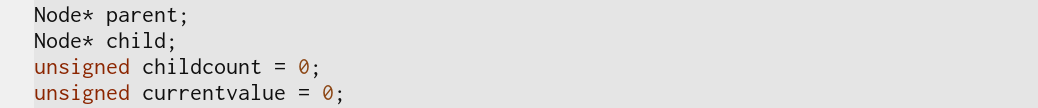
\includegraphics[width=\textwidth]{img/code2} \\
		\pause
		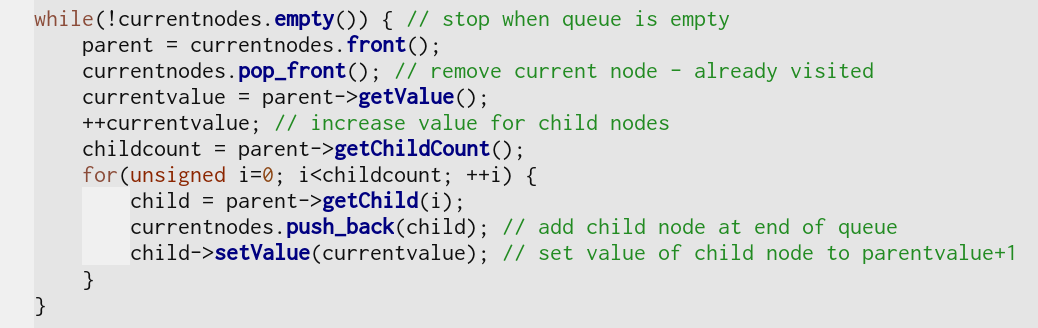
\includegraphics[width=\textwidth]{img/code3}
	\end{center}
\end{frame}
% \begin{frame}[fragile]
% 	\frametitle{Serial Code}
% 	\begin{lstlisting}[style=cpp]
% std::list<Node*> currentnodes;
% . . .
% Node* parent, child;
% unsigned childcount = currentvalue = 0;
% . . .
% while(!currentnodes.empty()) {
%   parent = currentnodes.front();
%   currentnodes.pop_front();
%   currentvalue = parent->getValue();
%   ++currentvalue;
%   childcount = parent->getChildCount();
%   for(unsigned i=0; i<childcount; ++i) {
%     child = parent->getChild(i);
%     currentnodes.push_back(child);
%     child->setValue(currentvalue);
%   }
% }
% \end{lstlisting}
% \end{frame}


%------------------------------------------------
\section{Parallelization}
%------------------------------------------------
% TODO: Kevin (3min)
\begin{frame}

\frametitle{Parallelization Ideas}
\begin{columns}
  \begin{column}{0.5\textwidth}
    \begin{itemize}
        \item Start in parallel at source nodes
        \item Spawn a new thread for every child node
        \item Synchronization needed when a node has multiple parents
        \item Performance dependent on topology of graph. Worst case $\mathcal{O}(N)$
    \end{itemize}
  \end{column}
  
  \begin{column}{0.5\textwidth}
    \begin{figure}[ht]
    %%TODO: Replace with more beautiful graph
    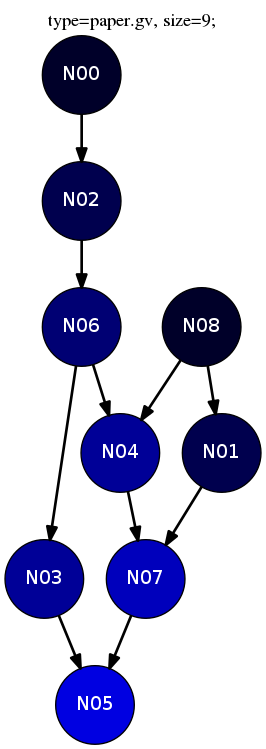
\includegraphics[width=0.4\textwidth]{img/paper}
    \end{figure}
  \end{column}
\end{columns}

\end{frame}

\begin{frame}
\frametitle{Synchronization ideas}
\begin{columns}
  \begin{column}{0.5\textwidth}
    \begin{itemize}
            \item Each thread enumerates the nodes it visits.
            \item If a node already has a number, take the higher number
    \end{itemize}
    \vspace{0.3cm}
    \begin{itemize}
            \item Problem: Multiple threads might ``follow'' each other.
            \item Idea: Only last thread arriving at a node may continue.
    \end{itemize}
  \end{column}
%   
  \begin{column}{0.5\textwidth}
    \begin{figure}[ht]
    %%TODO: Replace with more beautiful graph
    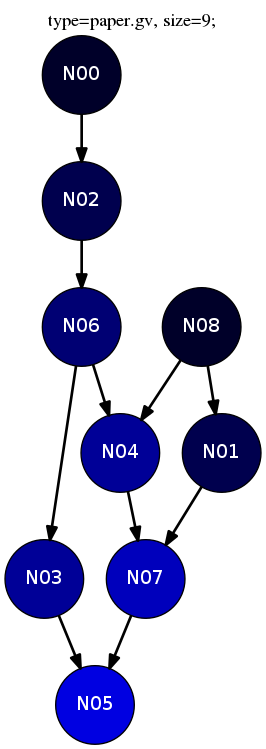
\includegraphics[width=0.4\textwidth]{img/paper}
    \end{figure}
  \end{column}
\end{columns}
\end{frame}

\begin{frame}
\frametitle{Hardware / Tools}
%TODO: Do we want to try MPI? Only makes things worse. We have no good way of fine-grained / coarse-grained parallelism
\begin{itemize}
        \item Shared memory parallelization
        \item OpenMP or C\texttt{++}11 threads.
        \item On Euler: 12-core Intel Xeon E5
        \item Intel Xeon Phi
\end{itemize}
\end{frame}

\begin{frame}
\frametitle{Challenges}
\begin{itemize}
	\item Task queue
	\item Find a way to cope with chain-like graphs.
	\item Optional goal: Find all possible topological sortings.
\end{itemize}
\end{frame}


\begin{frame}
\frametitle{Questions}
\begin{itemize}
	\item Up to how many execution units should we parallelize at least?
	\item From your experience, what are the main time-consuming, maybe unexpected obstacles when running on Intel Xeon Phi?
\end{itemize}
\end{frame}


\end{document} 
